\documentclass{beamer}

\usepackage{comment}
\usepackage{color}
\usepackage{listings}
\usepackage{verbatim}
\usepackage{multicol}
\usepackage{booktabs}
\usepackage{textpos}
\usepackage{graphicx}
\usepackage{graphics}
\definecolor{green}{RGB}{0,128,0}

\newcommand\gehcomment[1]{{{\color{orange} #1}}}
\newcommand\add[1]{{{\color{blue} #1}}}
\newcommand\remove[1]{\sout{{\color{red} #1}}}
\newcommand\codecomment[1]{{{\color{green} #1}}}
\newcommand\redcomment[1]{{{\color{red} #1}}}
\newcommand\bluecomment[1]{{{\color{blue} #1}}}
\newcommand\greencomment[1]{{{\color{green} #1}}}
\newcommand\magentacomment[1]{{{\color{magenta} #1}}}

\begin{document}
\title{CO2 Mineralization\ldots}
\author{Michael Nole}
\date{\today}

%\frame{\titlepage}

%-----------------------------------------------------------------------------
\section{Description of CO2 Mineralization Scenario}

\subsection{CO2 Mineralization Conceptual Model}

\frame{\frametitle{Description of CO2 Mineralization Scenario}

The ``CO2 Mineralization Scenario'' builds on the ``Injection Well Scenario'' and adds coupling between \bluecomment{SCO2 MODE} and \bluecomment{GIRT MODE} to model CO2 injection and mineralization.

This demonstration covers the following:

\begin{itemize}
  \small
  \item Modify the 2D heterogeneous model from the Injection Well short course problem to include chemistry coupling.
  \item Run the simulation.
  \item Visualize results in Paraview.
\end{itemize}
}

%-----------------------------------------------------------------------------
\section{Description of Input Deck}

%-----------------------------------------------------------------------------
\subsection{DESCRIPTION}

\begin{frame}[fragile,allowframebreaks]\frametitle{DESCRIPTION}

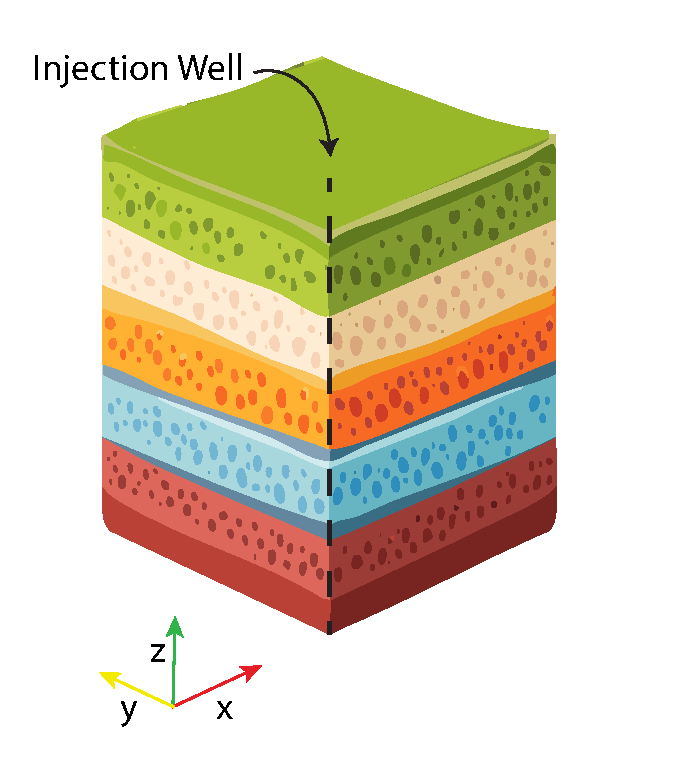
\includegraphics[height=3in]{injection-well-fig.pdf}

\newpage
\begin{itemize}
  \item 1. Initialize to hydrostatic conditions, isothermal temperature.
  \item 2. Add well model properties
  \item 3. Add geochemistry primary species, secondary species, minerals, and associated reaction rates.
  \item 4. Reference hanford.dat database
\end{itemize}

\end{frame}

%-----------------------------------------------------------------------------
\subsection{SIMULATION\_INJECTION\_WELL}

\begin{frame}[fragile,allowframebreaks]\frametitle{SIMULATION: CO2 Mineralization}

\begin{itemize}
\item Specify SCO2 flow mode
\item Add checkpointing
\end{itemize}


\begin{semiverbatim}
SIMULATION
  SIMULATION_TYPE SUBSURFACE
  PROCESS_MODELS
    SUBSURFACE_FLOW flow
      MODE SCO2
      OPTIONS
        ISOTHERMAL_TEMPERATURE 25.d0
        NO_STATE_TRANSITION_OUTPUT
      /
    /
    SUBSURFACE_TRANSPORT transport
      MODE GIRT
    /
\newpage
    WELL_MODEL well1
      OPTIONS
        FLOW_COUPLING FULLY_IMPLICIT
        TYPE HYDROSTATIC
      END
    END
  /
END

SUBSURFACE
CO2_DATABASE ../../../../../database/co2_sw.dat
...

\end{semiverbatim}

\end{frame}

%-----------------------------------------------------------------------------
\subsection{NUMERICAL METHODS}
\begin{frame}[fragile,allowframebreaks]\frametitle{NUMERICAL METHODS}

\begin{semiverbatim}
NUMERICAL_METHODS flow
  NEWTON_SOLVER
    USE_INFINITY_NORM_CONVERGENCE
    NUMERICAL_JACOBIAN
    MINIMUM_NEWTON_ITERATIONS 2
    CENTRAL_DIFFERENCE_JACOBIAN
    CONVERGE_ON_WELL_RESIDUAL
    RESIDUAL_SCALED_INF_TOL 1.d-4
  END

  TIMESTEPPER FLOW
    TIMESTEP_MAXIMUM_GROWTH_FACTOR 1.25
  END
END
\newpage
NUMERICAL_METHODS TRANSPORT
  TIMESTEPPER
    TS_ACCELERATION 16
  /
  NEWTON_SOLVER
    MAXIMUM_NUMBER_OF_ITERATIONS 100
  /
END

\end{semiverbatim}
\end{frame}

%-----------------------------------------------------------------------------
\subsection{WELL MODEL}
\begin{frame}[fragile,allowframebreaks]\frametitle{WELL MODEL}

\begin{semiverbatim}
WELLBORE_MODEL well1
  WELL_GRID
    WELL_TRAJECTORY
      SURFACE_ORIGIN 2.5d0 5.d0 -965.d0
      SEGMENT_DXYZ CASED 0.d0 0.d0 -15.04d0
      SEGMENT_DXYZ UNCASED 0.d0 0.d0 -176.9838d0
    /
  /

\newpage
  WELL
    DIAMETER 0.3d0
    FRICTION_COEFFICIENT 1.d0
    WELL_INDEX_MODEL PEACEMAN_3D
    SKIN_FACTOR 0.d0
  /

  USE_WELL_COUPLER

END
\newpage
WELL_MODEL_OUTPUT
  WELL_LIQ_PRESSURE
  WELL_GAS_PRESSURE
  WELL_LIQ_Q
  WELL_GAS_Q
/

\end{semiverbatim}
\end{frame}
%-----------------------------------------------------------------------------
\subsection{GRID}
\begin{frame}[fragile,containsverbatim]\frametitle{GRID}

\begin{itemize}
  \item Cartesian grid, converted to an unstructured implicit mesh.
\end{itemize}

\begin{semiverbatim}
GRID
  # nx=20 x ny=1 x nz=25
  TYPE UNSTRUCTURED mesh.ugi
END
\end{semiverbatim}

\end{frame}
%-----------------------------------------------------------------------------
\subsection{CHEMISTRY}
\begin{frame}[fragile,containsverbatim,allowframebreaks]\frametitle{CHEMISTRY}
\begin{semiverbatim}CHEMISTRY
  PRIMARY_SPECIES
    Al+++
    Ca++
    Fe++
    K+
    Mg++
    Mn++
    Na+
    SiO2(aq)
    Ti(OH)4(aq)
    H+
    CO2(aq)
    Cl-
    O2(aq)
  /
\newpage SECONDARY_SPECIES
    HCO3-
    OH-
    Al(OH)2+
    AlO2-
    AlOH++
    CO3--
    CaCO3(aq)
    CaHCO3+
    Fe+++
    Fe(OH)3(aq)
    Fe(OH)4-
    FeHCO3+
    HAlO2(aq)
    HSiO3-
\newpage
    MgCO3(aq)
    MgHCO3+
    MnCO3(aq)
    MnHCO3+
    MnOH+
    NaHCO3(aq)
    NaHSiO3(aq)
  /
\newpage
  ACTIVE_GAS_SPECIES
    GAS_TRANSPORT_IS_UNVETTED
    CO2(g)
  /
  PASSIVE_GAS_SPECIES
    CO2(g)
    O2(g)
  /
\newpage
  MINERALS
    Calcite
    Anatase
    Chalcedony
    Dawsonite
    Rhodochrosite
    Siderite
    Forsterite
    Fayalite
    Tephroite
    Wollastonite
    Enstatite
    Chrysotile
  /
\newpage
  MINERAL_KINETICS
    Calcite
      RATE_CONSTANT 5.01d-1 mol/cm^2-sec
      ACTIVATION_ENERGY 14.4 kJ/mol
    /
    Anatase
      RATE_CONSTANT 4.47d-9 mol/cm^2-sec
      ACTIVATION_ENERGY 37.9 kJ/mol
    /
    Chalcedony
      RATE_CONSTANT 5.89d-13 mol/cm^2-sec
      ACTIVATION_ENERGY 74.5 kJ/mol
    /
\newpage
    Dawsonite
      RATE_CONSTANT 1.0d-7 mol/cm^2-sec
      ACTIVATION_ENERGY 62.8 kJ/mol
    /
    Rhodochrosite
      RATE_CONSTANT 1.02d-3 mol/cm^2-sec
      ACTIVATION_ENERGY 21.0 kJ/mol
    /
    Siderite
      RATE_CONSTANT 1.02d-3 mol/cm^2-sec
      ACTIVATION_ENERGY 21.0 kJ/mol
    /
\newpage
    Forsterite
      PREFACTOR
      RATE_CONSTANT 5.41e-9 mol/cm^2-sec
      ACTIVATION_ENERGY 67.2d0
      PREFACTOR_SPECIES H+
         ALPHA 0.47d0
      /
      /
      PREFACTOR
      RATE_CONSTANT 2.29e-15 mol/cm^2-sec
      ACTIVATION_ENERGY 79.d0
      /
    /
\newpage
    Fayalite
      PREFACTOR
      RATE_CONSTANT 1.58e-13 mol/cm^2-sec
      ACTIVATION_ENERGY 98.4d0
      /
      PREFACTOR
      RATE_CONSTANT 1.58e-17 mol/cm^2-sec
      ACTIVATION_ENERGY 98.4d0
      /
    /
\newpage
    Tephroite
      PREFACTOR
      RATE_CONSTANT 1.5e-11 mol/cm^2-sec
      ACTIVATION_ENERGY 67.2d0
      PREFACTOR_SPECIES H+
        ALPHA 0.47d0
      /
      /
      PREFACTOR
      RATE_CONSTANT 2.51e-15 mol/cm^2-sec
      ACTIVATION_ENERGY 79.d0
      /
    /
\newpage
    Wollastonite
      PREFACTOR
      RATE_CONSTANT 5.27e-11 mol/cm^2-sec
      ACTIVATION_ENERGY 54.7d0
      PREFACTOR_SPECIES H+
        ALPHA 0.4d0
      /
      /
      PREFACTOR
      RATE_CONSTANT 1.32e-13 mol/cm^2-sec
      ACTIVATION_ENERGY 54.7d0
      /
    /
\newpage
    Enstatite
      PREFACTOR
      RATE_CONSTANT 9.55e-14 mol/cm^2-sec
      ACTIVATION_ENERGY 80.d0
      PREFACTOR_SPECIES H+
        ALPHA 0.6d0
      /
      /
      PREFACTOR
      RATE_CONSTANT 1.91e-13 mol/cm^2-sec
      ACTIVATION_ENERGY 80.d0
      /
    /
\newpage
    Chrysotile
      PREFACTOR
      RATE_CONSTANT 1.d-16 mol/cm^2-sec
      ACTIVATION_ENERGY 73.5d0
      /
      PREFACTOR
      RATE_CONSTANT 2.63e-18 mol/cm^2-sec
      ACTIVATION_ENERGY 73.5d0
      PREFACTOR_SPECIES H+
        ALPHA -0.23d0
      /
      /
    /
  /
\newpage
 DATABASE ../../../../../database/hanford.dat

  LOG_FORMULATION
  ACTIVITY_COEFFICIENTS TIMESTEP
  OUTPUT
    SECONDARY_SPECIES
    FREE_ION
    PH
    TOTAL
    MINERALS
  /
END
\end{semiverbatim}

\end{frame}
%-----------------------------------------------------------------------------
\subsection{FLUID\_PROPERTIES}
\begin{frame}[fragile,containsverbatim,allowframebreaks]\frametitle{Fluid Properties}

\begin{itemize}
  \item Define properties of water and gas
  \begin{itemize}
    \item Diffusion coefficients
    \item Equations of state
  \end{itemize}
\end{itemize}

\begin{semiverbatim}
FLUID_PROPERTY
  PHASE LIQUID
  DIFFUSION_COEFFICIENT 2.d-9
END

FLUID_PROPERTY
  PHASE GAS
  DIFFUSION_COEFFICIENT 2.d-5
END

\newpage

EOS WATER
  DENSITY IF97
  ENTHALPY IF97
  STEAM_DENSITY IF97
  STEAM_ENTHALPY IF97
  SATURATION_PRESSURE IF97
END

EOS GAS
  CO2_DATABASE ../../../../../database/co2_sw.dat
  HENRYS_CONSTANT DEFAULT
END

\end{semiverbatim}

\end{frame}
%-----------------------------------------------------------------------------
\subsection{MATERIAL\_PROPERTY}

\begin{frame}[fragile,containsverbatim,allowframebreaks]\frametitle{MATERIAL\_PROPERTY}

\begin{semiverbatim}
MATERIAL_PROPERTY caprock
  ID 1
  CHARACTERISTIC_CURVES caprock
  POROSITY 0.07
  TORTUOSITY 1.d0
  ROCK_DENSITY 2650.d0
  THERMAL_CONDUCTIVITY_DRY 2.d0
  THERMAL_CONDUCTIVITY_WET 2.18d0
  HEAT_CAPACITY 1000 J/kg-C
  PERMEABILITY
    PERM_ISO 5.6254628e-20
  /
  SOIL_COMPRESSIBILITY_FUNCTION LINEAR
  POROSITY_COMPRESSIBILITY 1.07618e-13
  SOIL_REFERENCE_PRESSURE 1.2d7
END \newpage
MATERIAL_PROPERTY Reservoir24
  ID 2
  CHARACTERISTIC_CURVES Reservoir24
  POROSITY 0.13
  TORTUOSITY 1.d0
  ROCK_DENSITY 2650.d0
  THERMAL_CONDUCTIVITY_DRY 2.d0
  THERMAL_CONDUCTIVITY_WET 2.18d0
  HEAT_CAPACITY 1000 J/kg-C
  PERMEABILITY
    PERM_ISO 1.9146312e-14
  /
  SOIL_COMPRESSIBILITY_FUNCTION LINEAR
  POROSITY_COMPRESSIBILITY 5.3809001e-14
  SOIL_REFERENCE_PRESSURE 1.2d7
END
\end{semiverbatim}
\newpage
\begin{itemize}
  \item +23 more reservoir units
\end{itemize}

\end{frame}

%-----------------------------------------------------------------------------
\subsection{CHARACTERISTIC\_CURVES}

\begin{frame}[fragile,containsverbatim, allowframebreaks]\frametitle{CHARACTERISTIC\_CURVES}

\begin{itemize}
\item Set Brooks-Corey parameters
\end{itemize}

\begin{semiverbatim}
CHARACTERISTIC_CURVES caprock
  SATURATION_FUNCTION BROOKS_COREY
    MAX_TRAPPED_GAS_SAT 0.2
    UNSATURATED_EXTENSION
    ALPHA 0.00001020408
    LAMBDA 0.8311
    LIQUID_RESIDUAL_SATURATION 0.0597
    MAX_CAPILLARY_PRESSURE 1.d9
  / 
\newpage
\begin{itemize}
\item BURDINE-BC relative permeability
\end{itemize}
  PERMEABILITY_FUNCTION BURDINE_BC_LIQ
    PHASE LIQUID
    LAMBDA 0.8311
    LIQUID_RESIDUAL_SATURATION 0.0597
  /
  PERMEABILITY_FUNCTION BURDINE_BC_GAS
    PHASE GAS
    LAMBDA 0.8311
    LIQUID_RESIDUAL_SATURATION 0.0597
    GAS_RESIDUAL_SATURATION 0.0597
  /
END
\end{semiverbatim}

\newpage

\begin{semiverbatim}
CHARACTERISTIC_CURVES Reservoir24
  SATURATION_FUNCTION BROOKS_COREY
    MAX_TRAPPED_GAS_SAT 0.2
    UNSATURATED_EXTENSION
    ALPHA 0.00008503401
    LAMBDA 0.8311
    LIQUID_RESIDUAL_SATURATION 0.0597
    MAX_CAPILLARY_PRESSURE 1.d9
  /
\newpage
  PERMEABILITY_FUNCTION BURDINE_BC_LIQ
    PHASE LIQUID
    LAMBDA 0.8311
    LIQUID_RESIDUAL_SATURATION 0.0597
  /
  PERMEABILITY_FUNCTION BURDINE_BC_GAS
    PHASE GAS
    LAMBDA 0.8311
    LIQUID_RESIDUAL_SATURATION 0.0597
    GAS_RESIDUAL_SATURATION 0.0597
  /
END
\end{semiverbatim}

\newpage
\begin{itemize}
  \item +23 more reservoir units
\end{itemize}

\end{frame}

%-----------------------------------------------------------------------------
\subsection{OUTPUT}

\begin{frame}[fragile,allowframebreaks]\frametitle{OUTPUT}

\begin{semiverbatim}

OUTPUT
  SNAPSHOT_FILE
    TIMES y 1.d-2 1.d-1 1.d0
    PERIODIC TIME 1.d0 y
    FORMAT HDF5
  /
  UNFILTER_NON_STATE_VARIABLES
\newpage  VARIABLES
   TEMPERATURE
   LIQUID_PRESSURE
   GAS_PRESSURE
   LIQUID_SATURATION
   GAS_SATURATION
   PRECIPITATE_SATURATION
   TRAPPED_GAS_SATURATION
   LIQUID_MASS_FRACTIONS
   GAS_MASS_FRACTIONS
   LIQUID_DENSITY
   GAS_DENSITY
   PERMEABILITY
   LIQUID_RELATIVE_PERMEABILITY
   GAS_RELATIVE_PERMEABILITY
  /
END
\end{semiverbatim}

\end{frame}

%-----------------------------------------------------------------------------
\subsection{TIME}

\begin{frame}[fragile]\frametitle{TIME}
\begin{semiverbatim}

TIME
  FINAL_TIME 1.d1 y
  INITIAL_TIMESTEP_SIZE 1.d-5 y
  MAXIMUM_TIMESTEP_SIZE 5.d-1 y
END

\end{semiverbatim}

\end{frame}

%-----------------------------------------------------------------------------
\subsection{REGION}

\begin{frame}[fragile,containsverbatim,allowframebreaks]\frametitle{REGION}

\begin{itemize}
  \item Delineate regions in the 2D domain for:
  \begin{itemize}
    \item east face
    \item caprock
    \item reservoir units
  \end{itemize}
\end{itemize}

\begin{semiverbatim}
REGION all
  COORDINATES
    0.d0    0.d0 -1157.024d0
    3048.d0 1.d3 -965.d0
  /
END
\newpage

REGION edge
  FACE EAST
  FILE mesh_ugi_east.ss
END

\newpage
REGION caprock
  COORDINATES
    0.d0    0.d0 -980.24
    3048.d0 1.d3 -965.9112d0
  /
END

REGION Reservoir24
  COORDINATES
    0.d0    0.d0 -983.288
    3048.d0 1.d3 -980.24
  /
END
\end{semiverbatim}

\begin{itemize}
  \item + 23 reservoir units
\end{itemize}

\end{frame}

%-----------------------------------------------------------------------------
\subsection{FLOW\_CONDITION}

\begin{frame}[fragile,allowframebreaks]\frametitle{FLOW\_CONDITION}

\begin{semiverbatim}
FLOW_CONDITION initial
  TYPE
    LIQUID_PRESSURE HYDROSTATIC
    CO2_MASS_FRACTION DIRICHLET
    SALT_MASS_FRACTION DIRICHLET
  /
  DATUM 0.d0 0.d0 -1040.892d0
  LIQUID_PRESSURE 1.234333924d7
  CO2_MASS_FRACTION 0.d0
  SALT_MASS_FRACTION 4.75d-2
END

\newpage
FLOW_CONDITION injection
  SYNC_TIMESTEP_WITH_UPDATE
  TYPE
    RATE MASS_RATE
  /
  # 1.0 MMT/yr for 2 years
  RATE LIST
    TIME_UNITS y
    DATA_UNITS kg/y kg/y kg/y
    0.d0 0.d0 1.d9 0.d0
    2.d0 0.d0 0.d0 0.d0
  /
END
\end{semiverbatim}

\end{frame}

%-----------------------------------------------------------------------------
\subsection{TRANSPORT\_CONDITION}

\begin{frame}[fragile,allowframebreaks]\frametitle{TRANSPORT\_CONDITION}

\begin{semiverbatim}
TRANSPORT_CONDITION background_conc
  TYPE ZERO_GRADIENT
  CONSTRAINT_LIST
    0.d0 initial_constraint
  /
END
\end{semiverbatim}

\end{frame}

%-----------------------------------------------------------------------------
\subsection{CONSTRAINT}

\begin{frame}[fragile,allowframebreaks]\frametitle{CONSTRAINT}

\begin{semiverbatim}
CONSTRAINT initial_constraint
  CONCENTRATIONS
    Al+++         8.48d-6  T
    Ca++          2.7d-5   T
    Fe++          1.72d-5  T
    K+            6.01d-5  T
    Mg++          4.53d-6  T
    Mn++          2.57d-7  T
    Na+           4.03d-3  T
    SiO2(aq)      1.28d-3  T
    Ti(OH)4(aq)   2.26d-10 T
    H+            10.      P
    CO2(aq)       1.d-4    T
    Cl-           1.d-6    T
    O2(aq)        1.d-10   T
  /
\newpage
  MINERALS
    Calcite 0.d0 1.d-2
    Anatase 0.d0 1
    Chalcedony 0.d0 1
    Dawsonite 0.d0 1
    Rhodochrosite 0.d0 1.d2
    Siderite 0.d0 1.d2
    Forsterite 0.03791 1
    Fayalite 0.075251 1
    Tephroite 0.400913 1.d2
    Wollastonite 0.401156 1.d2
    Enstatite 0.063452 1
    Chrysotile 0.02 1
  /
/
\end{semiverbatim}

\end{frame}

%-----------------------------------------------------------------------------
\subsection{INITIAL\_CONDITION}

\begin{frame}[fragile]\frametitle{INITIAL\_CONDITION}

\begin{semiverbatim}
INITIAL_CONDITION all
  FLOW_CONDITION initial
  \greencomment{TRANSPORT_CONDITION background_conc}
  REGION all
END

\end{semiverbatim}

\end{frame}

%-----------------------------------------------------------------------------
\subsection{BOUNDARY\_CONDITION}

\begin{frame}[fragile]\frametitle{BOUNDARY\_CONDITION}

\begin{semiverbatim}
WELL_COUPLER injection
  FLOW_CONDITION injection
  \greencomment{TRANSPORT_CONDITION background_conc}
  WELL well1
END

BOUNDARY_CONDITION edge
  FLOW_CONDITION initial
  \greencomment{TRANSPORT_CONDITION background_conc}
  REGION edge
END
\end{semiverbatim}

\end{frame}

%-----------------------------------------------------------------------------

\subsection{STRATA}

\begin{frame}[fragile]\frametitle{STRATA}

\begin{semiverbatim}

STRATA
  REGION caprock
  MATERIAL caprock
END

STRATA
  REGION Reservoir24
  MATERIAL Reservoir24
END

...

END_SUBSURFACE
\end{semiverbatim}

\end{frame}

%-----------------------------------------------------------------------------
\subsection{buoyant-flow.in}

\begin{frame}[fragile]\frametitle{Running PFLOTRAN}

\begin{semiverbatim}

> cd \$PFLOTRAN_DIR
> cd shortcourse/exercises/co2/sco2/co2-mineralization
> ./build_grid.sh
> pflotran -input_prefix co2-mineralization
> python co2-mineralization.py
> open co2-mass.png
> open minerals-formed.png
> open mineral-change.png
> paraview \&

\end{semiverbatim}

\end{frame}
\end{document}
